\documentclass[12pt,3p]{article}
\usepackage[utf8]{inputenc}
\usepackage[english]{babel}
 \usepackage[margin=0.5in]{geometry}
 \usepackage{amsmath}
 \usepackage{amssymb}
\usepackage{mathtools}
\usepackage{enumitem}
% For different colored text 
\usepackage{xcolor}
\usepackage[round,numbers]{natbib}
\usepackage[colorlinks = false]{hyperref}
\usepackage{graphicx}
\usepackage{subcaption}

\numberwithin{equation}{section}

\begin{document}

%====================================================================================
%====================================================================================
%====================================================================================
%====================================================================================
\title{Personal Notes on Paper: \\
	\large{A phase-field description of dynamic brittle fracture}}
\author{Borden, Verhoosel, Scott, Hughes, Landis}
\date{\vspace{-5ex}}
\maketitle

\tableofcontents
\newpage

%====================================================================================
%====================================================================================
%====================================================================================
\section{Definitions}
$\boldsymbol{\varepsilon}$: Strain Tensor \big[ Dimensionless \big] \\
$\psi_{e}$: Elastic energy density \big[ Energy / Volume \big] \\
$\lambda$ and $\mu$:  Lamé constants \\
$\Gamma (t)$: Set of cracks \\ 
$\Psi_{p o t}$: Potential energy of the body consisting of the elastic energy and the fracture energy \big[ Energy \big] \\
$G_c$: Fracture energy \big[ Energy / Area \big] \\
$\Psi_{k i n}$: Kinetic energy of the body \big[ Energy \big] \\
$L(\boldsymbol{u}, \boldsymbol{u}, \Gamma)$: Lagrangian \\ \\
%----
c(\textbf{x}, t): Phase field where 0 is fully damaged and 1 is fully undamaged \big[ Dimensionless \big] \\
$l_0$: model parameter controlling the width of the smooth approximation of the crack \big[ Length \big]\\
\textcolor{red}{what is k?}: model parameter  \\
$\psi_{e}^{+}$ and $\psi_{e}^{-}$: strain energies computed from the + and - components of the strain tensor [Energy/Volume] \\
$\boldsymbol{\varepsilon}^{+}$ and $\boldsymbol{\varepsilon}^{-}$: positive and negative components of the strain tensor \\
$\mathbf{P}$: orthonormal eigenvectors of the strain tensor \\
$\boldsymbol{\Lambda}$: diagonal matrix of principal strains \\
$ $: Mackauley bracket \\
$\kappa$: Bulk modulus \\
$\boldsymbol{\varepsilon}^{d e v}$: deviatoric strain tensor \\
$c (x,t)$: phase field [dimensionless] \\
$\mathcal{H}$: strain-history field [Energy / Volume]

%====================================================================================
%====================================================================================
%====================================================================================
\section{Formulation}

%====================================================================================
%====================================================================================
\subsection{Griffith's Theory of Brittle Fracture}
We have the typical strain equation
\begin{equation}\label{Strain}
\varepsilon_{i j} = u_{(i, j)} =\frac{1}{2}\left(\frac{\partial u_{i}}{\partial x_{j}}+\frac{\partial u_{j}}{\partial x_{i}}\right)
\end{equation}
Elastic energy density under the assumption of isotropic linear elasticity
\begin{equation}\label{ElasticEnergyDensity}
\psi_{e}(\boldsymbol{\varepsilon}) = \frac{1}{2} \lambda \varepsilon_{i i} \varepsilon_{j j}+\mu \varepsilon_{i j} \varepsilon_{i j}
\end{equation}
where $\lambda$ and $\mu$ are Lamé constants. The total potential energy of the body is the sum of the elastic energy and the fracture energy. 
\begin{equation}\label{PotEnergy}
\Psi_{p o t}(\boldsymbol{u}, \Gamma)=\int_{\Omega} \psi_{e}\left(\nabla^{s} \boldsymbol{u}\right) \mathrm{d} \boldsymbol{x}+\int_{\Gamma} \mathcal{G}_{c} \mathrm{d} \boldsymbol{x}
\end{equation}
\textcolor{red}{Note that $d \mathbf{x}$ is a little misleading because it can indicate both an area and a volume. Instead pay attention to the integral subscript notation.}The kinetic energy of the body is given by, 
\begin{equation}\label{KinEnergy}
\Psi_{k i n}(\dot{\boldsymbol{u}})=\frac{1}{2} \int_{\Omega} \rho \dot{u}_{i} \dot{u}_{i} \mathrm{d} \boldsymbol{x}
\end{equation}
The lagrangian for the discrete fracture problem is a combination of Eq. \ref{PotEnergy} and \ref{KinEnergy}, where we have grouped the volume terms and the area terms. 
\begin{equation}\label{Lagrangian}
\begin{aligned}
L(\boldsymbol{u}, \boldsymbol{u}, \Gamma) &=\Psi_{k i n}(\dot{\boldsymbol{u}})-\Psi_{p o t}(\boldsymbol{u}, \Gamma) \\
&=\int_{\Omega}\left[\frac{1}{2} \rho \dot{u}_{i} \dot{u}_{i}-\psi_{e}\left(\nabla^{s} \boldsymbol{u}\right)\right] \mathrm{d} \boldsymbol{x}-\int_{\Gamma} \mathcal{G}_{c} \mathrm{d} \boldsymbol{x}
\end{aligned}
\end{equation}

%====================================================================================
%====================================================================================
\subsection{Phase-field Approximation}
\textcolor{red}{These equations follow Miehe and Bourdin, citations 37 and 14 respectively.} \\ \\
Can approximate the fracture energy from a surface to a volume integral 
\begin{equation}\label{FractureSurfVol}
\int_{\Gamma} \mathcal{G}_{c} \mathrm{d} \boldsymbol{x} \approx \int_{\Omega} \mathcal{G}_{c}\left[\frac{(c-1)^{2}}{4 \ell_{0}}+\ell_{0} \frac{\partial c}{\partial x_{i}} \frac{\partial c}{\partial x_{i}}\right] \mathrm{d} \boldsymbol{x}
\end{equation}
where $\ell_0$ is a model parameter and $c(\boldsymbol{x}, t) \in[0,1]$ is the phase field where 0 is fully damaged. Again, the following equation introduces another model parameter, k, to model the loss of material stiffness in the failure zone. 
\begin{equation}\label{MatStiff}
\psi_{e}(\boldsymbol{\varepsilon}, c)=\left[(1-k) c^{2}+k\right] \psi_{e}^{+}(\boldsymbol{\varepsilon})+\psi_{e}^{-}(\boldsymbol{\varepsilon})
\end{equation}
where $\psi_{e}^{+}$ and $\psi_{e}^{-}$ are the strain energies computed from the positive and negative components of the strain tensor. \textcolor{red}{Why do we introduce k?} The spectral decomposition of strain is defined below \textcolor{red}{Why do we do this spectral decomposition?}
\begin{equation}\label{SpectDecStrain}
\boldsymbol{\varepsilon}=\mathbf{P} \mathbf{\Lambda} \mathbf{P}^{T}
\end{equation}
where, similarly, the positive and negative components of the strain tensor can be defined: 
\begin{equation}\label{PosNegStrain}
\begin{array}{l}
\boldsymbol{\varepsilon}^{+}=\mathbf{P} \mathbf{\Lambda}^{+} \mathbf{P}^{T} \\
\boldsymbol{\varepsilon}^{-}=\mathbf{P} \mathbf{\Lambda}^{-} \mathbf{P}^{T}
\end{array}
\end{equation}
where $\boldsymbol{\Lambda}^{+}=\operatorname{diag}\left(\left\langle\lambda_{1}\right\rangle,\left\langle\lambda_{2}\right\rangle,\left\langle\lambda_{3}\right\rangle\right)$ and 
$\boldsymbol{\Lambda}^{-}=\boldsymbol{\Lambda}-\boldsymbol{\Lambda}^{+}$. The Mackauley bracket is defined as usual, 
\begin{equation}\label{MacBracket}
\langle x\rangle=\left\{\begin{array}{ll}
x & x>0 \\
0 & x \leq 0
\end{array}\right.
\end{equation}
which essentially eliminates negative values. 
\begin{equation}
\begin{array}{l}
\psi_{e}^{+}(\boldsymbol{\varepsilon})=\frac{1}{2} \lambda\langle\operatorname{tr} \boldsymbol{\varepsilon}\rangle^{2}+\mu \operatorname{tr}\left[\left(\boldsymbol{\varepsilon}^{+}\right)^{2}\right] \\
\psi_{e}^{-}(\boldsymbol{\varepsilon})=\frac{1}{2} \lambda(\operatorname{tr} \boldsymbol{\varepsilon}-\langle\operatorname{tr} \boldsymbol{\varepsilon}\rangle)^{2}+\mu \operatorname{tr}\left[\left(\boldsymbol{\varepsilon}-\boldsymbol{\varepsilon}^{+}\right)^{2}\right]
\end{array}
\end{equation}
If we substitute these expressions into Eq. \ref{MatStiff}, we achieve:
\begin{align*}
\psi_{e}(\boldsymbol{\varepsilon}, c) &= \left[(1-k) c^{2}+k\right] \psi_{e}^{+}(\boldsymbol{\varepsilon})+\psi_{e}^{-}(\boldsymbol{\varepsilon}) \\
\psi_{e}(\boldsymbol{\varepsilon}, c) &= \left[(1-k) c^{2}+k\right] \bigg[ \frac{1}{2} \lambda\langle\operatorname{tr} \boldsymbol{\varepsilon}\rangle^{2}+\mu \operatorname{tr}\left[\left(\boldsymbol{\varepsilon}^{+}\right)^{2}\right] \bigg] +\frac{1}{2} \lambda(\operatorname{tr} \boldsymbol{\varepsilon}-\langle\operatorname{tr} \boldsymbol{\varepsilon}\rangle)^{2}+\mu \operatorname{tr}\left[\left(\boldsymbol{\varepsilon}-\boldsymbol{\varepsilon}^{+}\right)^{2}\right]
\end{align*}
This can be compared to the expression by Amor et al. [3]
\begin{equation}
\psi_{e}(\boldsymbol{\varepsilon}, c)=\left[(1-k) c^{2}+k\right]\left(\frac{\kappa}{2}\langle\mathrm{tr} \boldsymbol{\varepsilon}\rangle^{2}+\mu \operatorname{tr}\left[\left(\boldsymbol{\varepsilon}^{\mathrm{dev}}\right)^{2}\right]\right) + \frac{\kappa}{2}(\operatorname{tr} \boldsymbol{\varepsilon}-\langle\mathrm{tr} \boldsymbol{\varepsilon}\rangle)^{2}
\end{equation}
where $\kappa$ is the bulk modulus. \\
The deviatoric strain 
\begin{align*}
\boldsymbol{\varepsilon}^{\mathrm{dev}} &=
\begin{bmatrix}
\varepsilon_{11} & \varepsilon_{12} & \varepsilon_{13} \\
\varepsilon_{21} & \varepsilon_{22} & \varepsilon_{23} \\
\varepsilon_{31} & \varepsilon_{32} & \varepsilon_{33}
\end{bmatrix}
- \begin{bmatrix}
\varepsilon_m& 0 & 0 \\
0 & \varepsilon_m & 0 \\
0 & 0 & \varepsilon_m
\end{bmatrix} \\
&= 
\begin{bmatrix}
\varepsilon_{11} - \varepsilon_m & \varepsilon_{12} & \varepsilon_{13} \\
\varepsilon_{21} & \varepsilon_{22} - \varepsilon_m & \varepsilon_{23} \\
\varepsilon_{31} & \varepsilon_{32} & \varepsilon_{33} - \varepsilon_m
\end{bmatrix}
\end{align*}
We're only interested in the diagonals of the square. 
\begin{align*}
\langle \boldsymbol{\varepsilon}^{\mathrm{dev}} \rangle^2
&= 
\begin{bmatrix}
( \varepsilon_{11} - \varepsilon_m)^2 + \varepsilon_{12} \varepsilon_{21}  + \varepsilon_{13} \varepsilon_{31} & ? & ? \\
? & \varepsilon_{21} \varepsilon_{12}  + ( \varepsilon_{22} - \varepsilon_m)^2 +  \varepsilon_{23} \varepsilon_{32}  &? \\
? & ? & \varepsilon_{31} \varepsilon_{13} + \varepsilon_{32} \varepsilon_{23} + ( \varepsilon_{33} - \varepsilon_m)^2 
\end{bmatrix}
\end{align*}
The trace of this is therefore
\begin{align*}
\mathrm{tr} \langle \boldsymbol{\varepsilon}^{\mathrm{dev}} \rangle^2 
&= ( \varepsilon_{11} - \varepsilon_m)^2 + \varepsilon_{12} \varepsilon_{21}  + \varepsilon_{13} \varepsilon_{31} + \varepsilon_{21} \varepsilon_{12}  + ( \varepsilon_{22} - \varepsilon_m)^2 +  \varepsilon_{23} \varepsilon_{32}  + \varepsilon_{31} \varepsilon_{13} + \varepsilon_{32} \varepsilon_{23}  +  \varepsilon_{32} \varepsilon_{23} + ( \varepsilon_{33} - \varepsilon_m)^2 \\
&= ( \varepsilon_{11} - \varepsilon_m)^2  + ( \varepsilon_{22} - \varepsilon_m)^2 + (\varepsilon_{33} - \varepsilon_m)^2 + 2 \varepsilon_{12} \varepsilon_{21}  + 2 \varepsilon_{13} \varepsilon_{31} + 2 \varepsilon_{23} \varepsilon_{32} \\
&= 
\varepsilon_{11}^2 - 2 \varepsilon_{11} \varepsilon_{m} + \varepsilon_m^2 
+ \varepsilon_{22}^2 - 2 \varepsilon_{22} \varepsilon_{m} + \varepsilon_m^2 
+ \varepsilon_{33}^2 - 2 \varepsilon_{33} \varepsilon_{m} + \varepsilon_m^2 
+ 2 \varepsilon_{12} \varepsilon_{21}  + 2 \varepsilon_{13} \varepsilon_{31} + 2 \varepsilon_{23} \varepsilon_{32} \\
&= 
(\varepsilon_{11}^2 + \varepsilon_{22}^2 + \varepsilon_{33}^2 )
- 2 \varepsilon_{m} ( \varepsilon_{11}  + \varepsilon_{22} + \varepsilon_{33} ) 
+ 3 \varepsilon_m^2 
+ 2 ( \varepsilon_{12} \varepsilon_{21}  + \varepsilon_{13} \varepsilon_{31} + \varepsilon_{23} \varepsilon_{32})  \\
&= 
\mathrm{tr} \langle \boldsymbol{\varepsilon} \rangle^2 - 2 \frac{1}{3} \langle \mathrm{tr} \boldsymbol{\varepsilon} \rangle  \langle \mathrm{tr} \boldsymbol{\varepsilon} \rangle 
+ 3 \frac{1}{9}  \langle \mathrm{tr} \boldsymbol{\varepsilon} \rangle^2  
+ 2 ( \varepsilon_{12}^2 + \varepsilon_{13}^2 + \varepsilon_{23}^2)  \\
&= 
\mathrm{tr} \langle \boldsymbol{\varepsilon} \rangle^2 - \frac{2}{3} \langle \mathrm{tr} \boldsymbol{\varepsilon} \rangle^2 
+ \frac{1}{3}  \langle \mathrm{tr} \boldsymbol{\varepsilon} \rangle^2  
+ 2 ( \varepsilon_{12}^2 + \varepsilon_{13}^2 + \varepsilon_{23}^2) \\
\mathrm{tr} \langle \boldsymbol{\varepsilon}^{\mathrm{dev}} \rangle^2 &= 
\mathrm{tr} \langle \boldsymbol{\varepsilon} \rangle^2 - \frac{1}{3} \langle \mathrm{tr} \boldsymbol{\varepsilon} \rangle^2 + 2 ( \varepsilon_{12}^2 + \varepsilon_{13}^2 + \varepsilon_{23}^2)  
\end{align*}
where we have recognized
\begin{align*}
\varepsilon_{m} = \frac{1}{3} \langle \varepsilon_{11} + \varepsilon_{22} + \varepsilon_{33} \rangle = \frac{1}{3} \langle \mathrm{tr} \boldsymbol{\varepsilon} \rangle
\end{align*}
The most obvious difference is that our expression has an extra term, the last term. In the Amor et al. [3] model, expansive volumetric strain energy, as measured by $\langle\text { tr } \boldsymbol{\varepsilon}\rangle,$ and deviatoric strain energy, are subjected to damage, but not compressive volumetric strain energy. We note a difference of this model compared with the model we use is that, all three principal strains could be negative, but the deviatoric strain energy would experience damage, unlike the model we use. However, the intent of both models is similar, which is to maintain resistance in compression and during crack closure. \\ \\
Substitution of Eq. \ref{MatStiff} and \ref{FractureSurfVol} into Eq. \ref{Lagrangian} yields this full expression for the lagrangian.  
\begin{equation}\label{FullLagrangian}
\begin{aligned}
L_{\varepsilon}(\boldsymbol{u}, \dot{\boldsymbol{u}}, c)=& \int_{\Omega}\left(\frac{1}{2} \rho \dot{u}_{i} \dot{u}_{i}-\left[(1-k) c^{2}+k\right] \psi_{\mathrm{e}}^{+}\left(\nabla^{s} \boldsymbol{u}\right)-\psi_{\mathrm{e}}^{-}\left(\nabla^{s} \boldsymbol{u}\right)\right) \mathrm{d} \boldsymbol{x} 
&-\int_{\Omega} \mathcal{G}_{c}\left[\frac{(c-1)^{2}}{4 \ell_{0}}+\ell_{0} \frac{\partial c}{\partial x_{i}} \frac{\partial c}{\partial x_{i}}\right] \mathrm{d} \boldsymbol{x}
\end{aligned}
\end{equation}
We can use the Euler Lagrange Equations to arrive at the equations of motion, which requires us to calculate two partials (see notes below). Start by rewriting Eq. \ref{FullLagrangian}
\begin{align*}
L_{\varepsilon}(\boldsymbol{u}, \dot{\boldsymbol{u}}, c) &= 
\int_{\Omega} \frac{1}{2} \rho \frac{\partial u_i}{\partial t} \frac{\partial u_i}{\partial t} \mathrm{d} \boldsymbol{x} 
- \int_{\Omega} \left[(1-k) c^{2} + k \right] \psi_{\mathrm{e}}^{+} \left(\nabla^{s} \boldsymbol{u} \right) \mathrm{d} \boldsymbol{x} 
- \int_{\Omega} \psi_{\mathrm{e}}^{-} \left(\nabla^{s} \boldsymbol{u}\right) \mathrm{d} \mathbf{x} \\
&-\int_{\Omega} \mathcal{G}_{c} \frac{(c-1)^{2}}{4 \ell_{0}} \mathrm{d} \boldsymbol{x} 
- \int_{\Omega} \mathcal{G}_{c} \ell_{0} \frac{\partial c}{\partial x_{i}} \frac{\partial c}{\partial x_{i}} \mathrm{d} \boldsymbol{x}
\end{align*}
Next, note that the definition for the Cauchy stress tensor: 
\begin{equation}\label{CauchyStress}
\sigma_{i j}=\left[(1-k) c^{2}+k\right] \frac{\partial \psi_{\mathrm{e}}^{+}}{\partial \varepsilon_{i j}}+\frac{\partial \psi_{\mathrm{e}}^{-}}{\partial \varepsilon_{i j}}
\end{equation}
Since we are trying to derive the Equilibrium equation, we note that 
\begin{align}\label{DerCauchyStress}
\begin{split}
\frac{\partial \sigma_{i j}}{\partial x_j} &= 
\left[(1-k) c^{2}+k\right] \frac{\partial}{\partial x_j} \bigg( \frac{\partial \psi_{\mathrm{e}}^{+}}{\partial \varepsilon_{i j}} \bigg) + \frac{\partial}{\partial x_j} \bigg( \frac{\partial \psi_{\mathrm{e}}^{-}}{\partial \varepsilon_{i j}} \bigg) \\
\frac{\partial \sigma_{i j}}{\partial x_j} &= 
\left[(1-k) c^{2}+k\right] \frac{\partial \psi_{\mathrm{e}}^{+}}{\partial u_i} + \frac{\partial \psi_{\mathrm{e}}^{-}}{\partial u_i}
\end{split}
\end{align}
The independent fields are the vector field of displacement, $\mathbf{u} (\mathbf{x}, t)$ and the scalar phase-field of damage, $c (\mathbf{x}, t)$. First, we can take the partial derivative with respect to the displacement field:
\begin{align*}
\frac{\partial L_{\varepsilon}}{\partial \mathbf{u}} &= 
\int_{\Omega} \frac{1}{2} \rho \frac{\partial}{\partial \mathbf{u}} \bigg( \frac{\partial u_i}{\partial t} \frac{\partial u_i}{\partial t} \bigg) \mathrm{d} \boldsymbol{x} 
- \int_{\Omega} \left[(1-k) c^{2} + k \right] \frac{\partial \psi_{\mathrm{e}}^{+} \left(\nabla^{s} \boldsymbol{u} \right)}{\partial \mathbf{u}} \mathrm{d} \boldsymbol{x} 
- \int_{\Omega} \frac{\partial \psi_{\mathrm{e}}^{-} \left(\nabla^{s} \boldsymbol{u}\right)}{\partial \mathbf{u}} \mathrm{d} \boldsymbol{x} \\
&= \int_{\Omega} \frac{1}{2} \rho \bigg( 2 \frac{\partial^2 u_i}{\partial t^2} \bigg) \mathrm{d} \boldsymbol{x} 
- \int_{\Omega} \bigg( \left[(1-k) c^{2} + k \right] \frac{\partial \psi_{\mathrm{e}}^{+} }{\partial \mathbf{u}} + \frac{\partial \psi_{\mathrm{e}}^{-}}{\partial \mathbf{u}} \bigg) \mathrm{d} \boldsymbol{x}  \quad \text{Recognize Eq. \ref{DerCauchyStress}} \\
&= \int_{\Omega} \rho \frac{\partial^2 u_i}{\partial t^2} \mathrm{d} \boldsymbol{x} 
- \int_{\Omega} \frac{\partial \sigma_{i j}}{\partial x_j} \mathrm{d} \boldsymbol{x} \\
\frac{\partial L_{\varepsilon}}{\partial u_i} &= \int_{\Omega} \bigg( \rho \frac{\partial^2 u_i}{\partial t^2} - \frac{\partial \sigma_{i j}}{\partial x_j} \bigg) \mathrm{d} \boldsymbol{x}
\end{align*}
We can already see the equilibrium equation as the section in parenthesis is equivalent to zero
\begin{equation}\label{EqmEq}
\frac{\partial \sigma_{i j}}{\partial x_j} = \rho \frac{\partial^2 u_i}{\partial t^2} 
\end{equation}
Secondly, we can take the partial derivative with respect to the damage field. 
\begin{align*}
\frac{\partial L_{\varepsilon}}{\partial c} &= 
- \frac{\partial}{\partial c} \int_{\Omega} \left[(1-k) c^{2} + k \right] \psi_{\mathrm{e}}^{+} \mathrm{d} \boldsymbol{x} 
- \frac{\partial}{\partial c} \int_{\Omega} \mathcal{G}_{c} \frac{(c-1)^{2}}{4 \ell_{0}} \mathrm{d} \boldsymbol{x} 
- \frac{\partial}{\partial c} \int_{\Omega} \mathcal{G}_{c} \ell_{0} \frac{\partial c}{\partial x_{i}} \frac{\partial c}{\partial x_{i}} \mathrm{d} \boldsymbol{x} \\
&= 
-\int_{\Omega} 2 (1 - k) c \psi_{\mathrm{e}}^{+} \mathrm{d} \boldsymbol{x}
- \int_{\Omega} \mathcal{G}_{c} \frac{2 (c-1)}{4 \ell_{0}} \mathrm{d} \boldsymbol{x} 
- \int_{\Omega} \mathcal{G}_{c} \ell_{0} \frac{\partial}{\partial c} \bigg( \frac{\partial c}{\partial x_{i}} \frac{\partial c}{\partial x_{i}} \bigg) \mathrm{d} \boldsymbol{x} \\
&= 
- \int_{\Omega} 2 (1 - k) c \psi_{\mathrm{e}}^{+} \mathrm{d} \boldsymbol{x}
- \int_{\Omega} \mathcal{G}_{c} \frac{(c-1)}{2 \ell_{0}} \mathrm{d} \boldsymbol{x} 
- \int_{\Omega} 2 \mathcal{G}_{c} \ell_{0} \frac{\partial c}{\partial x_i} \mathrm{d} \boldsymbol{x} 
\end{align*}
Now if we group these similarly: 
\begin{align*}
0 &= - 2 (1 - k) c \psi_{\mathrm{e}}^{+} - \mathcal{G}_{c} \frac{(c-1)}{2 \ell_{0}} - 2 \mathcal{G}_{c} \ell_{0} \frac{\partial c}{\partial x_i} \quad \text{multiply through by } -2 \ell_0 / \mathcal{G}_c \\
0 &= 4 \frac{\ell_0 (1 - k) c \psi_{\mathrm{e}}^{+}}{\mathcal{G}_c} + (c-1) + 4 \ell_{0}^2 \frac{\partial^2 c}{\partial x_i^2} \\
1 &= 4 \frac{\ell_0 (1 - k) c \psi_{\mathrm{e}}^{+}}{\mathcal{G}_c} + c + 4 \ell_{0}^2 \frac{\partial^2 c}{\partial x_i^2} \\
1 &= \bigg( \frac{4 \ell_0 (1 - k) \psi_{\mathrm{e}}^{+}}{\mathcal{G}_c} + 1 \bigg) c + 4 \ell_{0}^2 \frac{\partial^2 c}{\partial x_i^2}
\end{align*}
Therefore, we arrive at the strong form equations of motion: 
\begin{align}\label{EqMotion}
\begin{split}
\frac{\partial \sigma_{i j}}{\partial x_j} = \rho \frac{\partial^2 u_i}{\partial t^2} \quad \text{on }& \Omega \times [0, T]\\
\bigg( \frac{4 \ell_0 (1 - k) \psi_{\mathrm{e}}^{+}}{\mathcal{G}_c} + 1 \bigg) c + 4 \ell_{0}^2 \frac{\partial^2 c}{x_i^2} = 1 \quad \text{on }& \Omega \times [0, T]
\end{split}
\end{align}
which can be solved to find the displacement and phase field. \\ \\
\textcolor{red}{There is a sign difference between this result and Eq. 18}
\begin{align*}
\bigg( \frac{4 \ell_0 (1 - k) \psi_{\mathrm{e}}^{+}}{\mathcal{G}_c} + 1 \bigg) c - 4 \ell_{0}^2 \frac{\partial^2 c}{\partial x_i^2} = 1 \quad \text{on }& \Omega \times [0, T]
\end{align*}
We can introduce a strain-history field, $\mathcal{H}$, which satisfies the KKT conditions for loading and unloading.
\begin{align}
\begin{split}
\psi_{e}^{+}-\mathcal{H} &\leqslant 0 \\
\dot{\mathcal{H}} &\geqslant 0 \\
\dot{\mathcal{H}}\left(\psi_{e}^{+} - \mathcal{H}\right) &= 0
\end{split}
\end{align}
Substitute $\mathcal{H}$ for $\psi_{e}^{+}$ in Eq. \ref{EqMotion}
\begin{align}\label{EqMotionHistoryField}
\begin{split}
\frac{\partial \sigma_{i j}}{\partial x_j} = \rho \frac{\partial^2 u_i}{\partial t^2} \quad \text{on }& \Omega \times [0, T]\\
\bigg( \frac{4 \ell_0 (1 - k) \mathcal{H}}{\mathcal{G}_c} + 1 \bigg) c - 4 \ell_{0}^2 \frac{\partial^2 c}{\partial x_i^2} = 1 \quad \text{on }& \Omega \times [0, T]
\end{split}
\end{align}
\textcolor{red}{Boundary conditions are listed here in the text }
%-------
\paragraph{Notes on the Euler-Lagrange Equations \\} 
Say we're given an equation in the form where the real argument is t, 
\begin{equation*}
S (\mathbf{q}) = \int_{a}^{b} L (t, \mathbf{q}(t), \dot{\mathbf{q}} (t)) dt 
\end{equation*}
We can write an equation in the form
\begin{equation*}
\frac{\partial L(t, \mathbf{q}(t), \dot{\mathbf{q}} (t))}{\partial \mathbf{q} (t)}  - \frac{d}{dt} \frac{\partial L(t, \mathbf{q}(t), \dot{\mathbf{q}} (t))}{\partial \dot{\mathbf{q}} (t)} = 0
\end{equation*}

%====================================================================================
%====================================================================================
\subsection{Analytical solutions of the 1D quasi-static problem}
If we consider a 1D problem, ignore all temporal derivatives, and assume k = 0, we obtain from Eq. \ref{EqMotion}. 
\begin{align*}
\frac{\partial \sigma_{i j}}{\partial x_j} &= \rho \frac{\partial^2 u_i}{\partial t^2} \\
\frac{d \boldsymbol{\sigma}}{dx} &= 0
\end{align*}
The second equation yields: 
\begin{align*}
\bigg( \frac{4 \ell_0 (1 - k) \mathcal{H}}{\mathcal{G}_c} + 1 \bigg) c - 4 \ell_{0}^2 \frac{\partial^2 c}{\partial x_i^2} &= 1 \\
\bigg( \frac{4 \ell_0 (1 - k) \mathcal{H}}{\mathcal{G}_c} + 1 \bigg) c - 4 \ell_{0}^2 \frac{d^2 c}{d x^2} &= 1 \\
\bigg( \frac{4 \ell_0 \mathcal{H}}{\mathcal{G}_c} + 1 \bigg) c - 4 \ell_{0}^2 \frac{d^2 c}{d x^2} &= 1\end{align*}
Combined, 
\begin{align}\label{1DQuasiStaticMotion}
\begin{split}
\frac{d \boldsymbol{\sigma}}{dx} &= 0 \\
\bigg( \frac{4 \ell_0 \mathcal{H}}{\mathcal{G}_c} + 1 \bigg) c - 4 \ell_{0}^2 \frac{d^2 c}{d x^2} &= 1 
\end{split}
\end{align}
We can also simplify Eq. \ref{MatStiff} based on the fact that k = 0 and assuming that the strain field is non-negative $\psi_{e}^{-}  = 0$
\begin{align*}
\psi_{e}(\boldsymbol{\varepsilon}, c) &=\left[(1-k) c^{2} + k\right] \psi_{e}^{+}(\boldsymbol{\varepsilon})+\psi_{e}^{-}(\boldsymbol{\varepsilon}) \\
\psi_{e}(\boldsymbol{\varepsilon}, c) &= c^{2} \psi_{e}^{+} (\boldsymbol{\varepsilon}) \quad \text{where }  \psi_{e}^{+} = \frac{1}{2} E \boldsymbol{\varepsilon}^2 \\
\psi_{e}(\boldsymbol{\varepsilon}, c) &= \frac{1}{2} c^{2} E \boldsymbol{\varepsilon}^2 
\end{align*}
We can simplify Eq. \ref{CauchyStress} based on the simplification for Eq. \ref{MatStiff}
\begin{align*}
\sigma_{i j} &= \left[(1-k) c^{2}+k\right] \frac{\partial \psi_{\mathrm{e}}^{+}}{\partial \varepsilon_{i j}} + \frac{\partial \psi_{\mathrm{e}}^{-}}{\partial \varepsilon_{i j}} \\
\boldsymbol{\sigma} &= c^2 \frac{\partial \psi_{\mathrm{e}}^{+}}{\partial \boldsymbol{\varepsilon}} \quad \text{where }  \psi_{e}^{+} = \frac{1}{2} E \boldsymbol{\varepsilon}^2 \\
\boldsymbol{\sigma} &= c^2 \frac{\partial}{\partial \boldsymbol{\varepsilon}} \bigg( \frac{1}{2} E \boldsymbol{\varepsilon}^2 \bigg) \\
\boldsymbol{\sigma} &= c^2 E \boldsymbol{\varepsilon}
\end{align*}
The stress is constant over the domain. 
\begin{equation}\label{HomogStress}
\boldsymbol{\sigma} = c^2 E \boldsymbol{\varepsilon}
\end{equation}

%====================================================================================
\subsubsection{Homogeneous Solution}
The homogeneous solution is examined by ignoring all spatial derivatives of c. We can start with Eq. \ref{1DQuasiStaticMotion}
\begin{align*}
\bigg( \frac{4 \ell_0 \mathcal{H}}{\mathcal{G}_c} + 1 \bigg) c - 4 \ell_{0}^2 \frac{d^2 c}{d x^2} &= 1 \\
\bigg( \frac{4 \ell_0 \mathcal{H}}{\mathcal{G}_c} + 1 \bigg) c_{\mathrm{hom}} &= 1 \quad \text{Rearrange for } c_{\mathrm{hom}} \\
c_{\mathrm{hom}} &= \bigg( \frac{4 \ell_0 \mathcal{H}}{\mathcal{G}_c} + 1 \bigg)^{-1}
\end{align*}
We actually achieve two results 
\begin{equation}\label{CHom}
c_{\mathrm{hom}}=\left\{\begin{array}{ll}
\left(\frac{2 \ell_{0} E}{\mathcal{G}_{c}} \boldsymbol{\varepsilon}_{\mathrm{hom}}^{2}+1\right)^{-1} & \mathcal{H}  = \psi_{e}^{+} = \frac{1}{2} E \boldsymbol{\varepsilon}^2 \\
\left(\frac{4 \ell_{0}}{\mathcal{G}_{c}} \mathcal{H}+1\right)^{-1} & \mathcal{H} > \psi_{e}^{+}
\end{array}\right.
\end{equation}
where $c_{\mathrm{hom}}$ and $\boldsymbol{\varepsilon}_{\mathrm{hom}}$ are the homogenous phase-field and strain respectively. Substitute Eq. \ref{CHom} into Eq. \ref{HomogStress}
\begin{equation}
\sigma_{\mathrm{hom}}=\left\{\begin{array}{ll}
\left(\frac{2 \ell_{0} E}{\mathcal{G}_{c}} \varepsilon_{\mathrm{hom}}^{2}+1\right)^{-2} E \varepsilon_{\mathrm{hom}} & \mathcal{H} = \psi_{e}^{+} \\
\left(\frac{4 \ell_{0}}{\mathcal{G}_{c}} \mathcal{H}+1\right)^{-2} E \varepsilon_{\mathrm{hom}} & \mathcal{H} > \psi_{e}^{+}
\end{array}\right.
\end{equation}

\subsubsection{Non-Homogeneous Solution}
Start with Eq. \ref{1DQuasiStaticMotion} where we know that $\mathcal{H} = \frac{1}{2} E \varepsilon^2$
\begin{align*}
\bigg(\frac{4 \ell_0 \mathcal{H}}{\mathcal{G}_c} + 1 \bigg) c - 4 \ell_0^2 \frac{d^2 c }{d x^2} &= 1 \\
\bigg(\frac{2 \ell_0 E \varepsilon^2}{\mathcal{G}_c} + 1 \bigg) c - 4 \ell_0^2 \frac{d^2 c }{d x^2} &= 1 \quad \text{where } \sigma = c^2 E \varepsilon \rightarrow \frac{\sigma^2}{c^4 E} = E \varepsilon^2 \\
\bigg(\frac{2 \ell_0 \sigma^2}{c^4 E \mathcal{G}_c} + 1 \bigg) c - 4 \ell_0^2 \frac{d^2 c }{d x^2} -1 &= 0 \quad \text{divide by 2} \\
\bigg(\frac{\ell_0 \sigma^2}{c^4 E \mathcal{G}_c} + \frac{1}{2} \bigg) c - 2 \ell_0^2 \frac{d^2 c }{d x^2} - \frac{1}{2} &= 0 \quad \text{multiply by } dc/dx \\
\frac{dc}{dx} \bigg[ \bigg(\frac{\ell_0 \sigma^2}{c^4 E \mathcal{G}_c} + \frac{1}{2} \bigg) c - 2 \ell_0^2 \frac{d^2 c }{d x^2} - \frac{1}{2} \bigg] &= 0 \\
\frac{d}{dx} \bigg[ \bigg(\frac{\ell_0 \sigma^2}{c^3 E \mathcal{G}_c} + \frac{c}{2} \bigg) c - 2 c \ell_0^2 \frac{d^2 c }{d x^2} - \frac{c}{2} \bigg] &= 0 \\
\frac{d}{dx} \bigg[ \frac{\ell_0 \sigma^2}{c^2 E \mathcal{G}_c} + \frac{c^2}{2}- 2 c \ell_0^2 \frac{d^2 c }{d x^2} - \frac{c}{2} \bigg] &= 0 \\
\end{align*}

%\begin{figure}[h]
%    \centering
%    \begin{subfigure}[b]{0.45\textwidth}
%        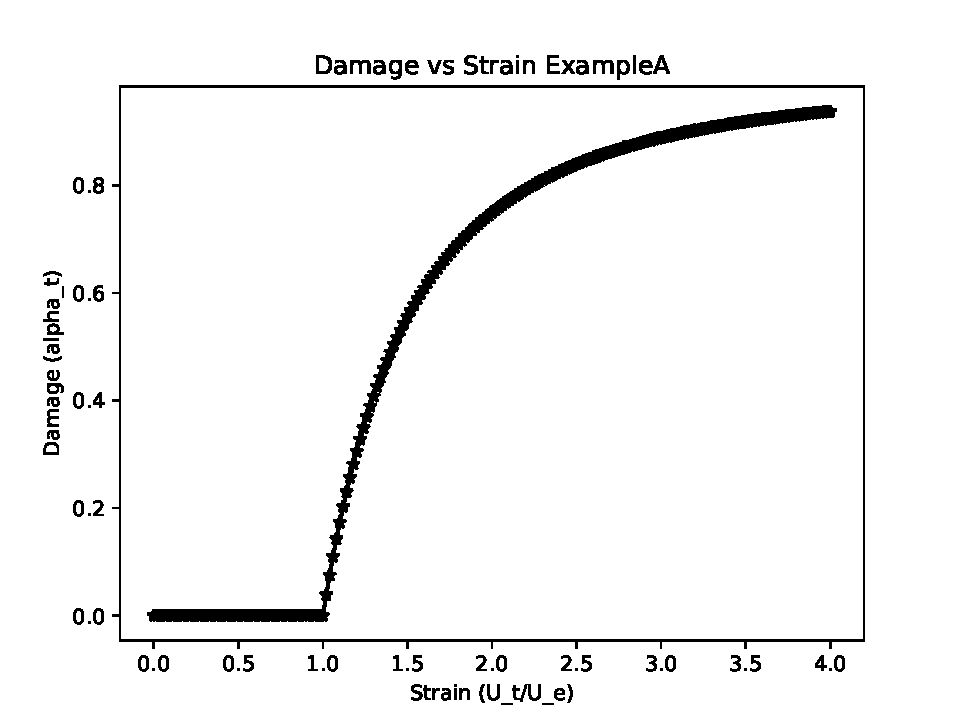
\includegraphics[width=\textwidth]{Images/A_damage_strain_dim.pdf}
%    \end{subfigure}
%    \quad %add desired spacing between images, e. g. ~, \quad, \qquad, \hfill etc. 
%    \begin{subfigure}[b]{0.45\textwidth}
%        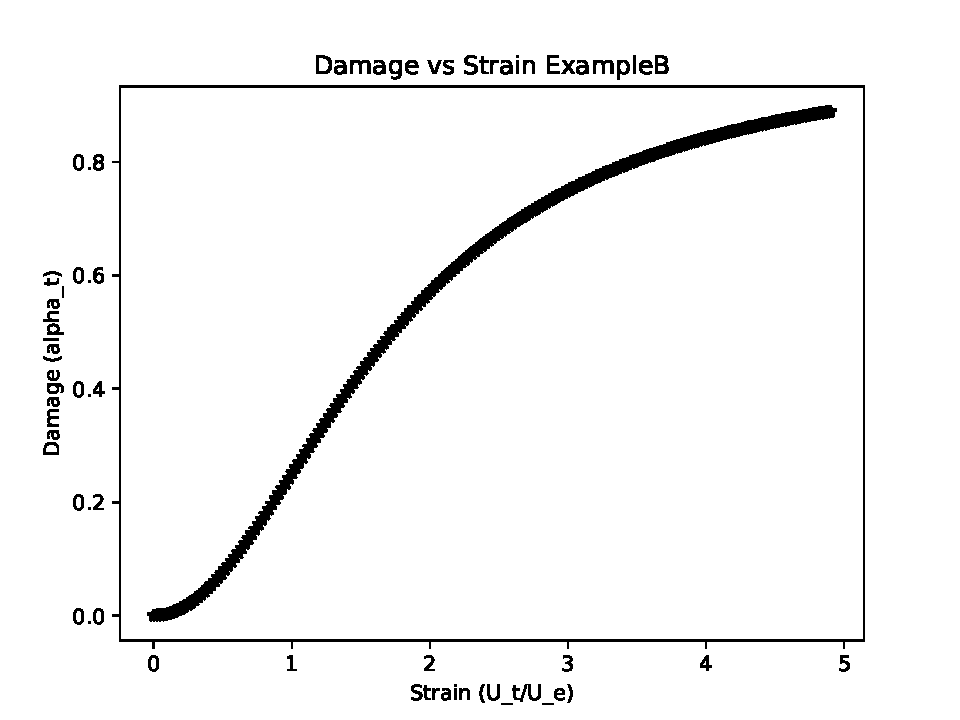
\includegraphics[width=\textwidth]{Images/B_damage_strain_dim.pdf}
%    \end{subfigure}
%    \caption{Damage vs strain property of the homogenous solution for A) example 1 and B) example 2}
%\end{figure}


\end{document}